\chapter{トランスポート層(その1) トランスポート層の概論}

アプリケーション層にサービスをするのが、トランスポート層です。トランスポート層は、ここまでで確実な通信を提供するのが役目という説明をしました。では、どうやって確実な通信をしているのか、そして、確実な通信をしなくていいときはどうしているおか、それを見てみることにします。

\section{トランスポート層とはなにか}

トランスポート層は、TCP/IPにおいて、アプリケーション層とインターネットプロと固陋そうに挟まれたレイヤである。その位置でわかるように、インターネット層のサービスを通信路として利用するレイヤである。そして、アプリケーション層にサービスを提供するレイヤである。

\subsection{トランスポート層の通信相手}
まず、トランスポートスの通信相手はなんだろうか。それは、通信の相手となるホストの上で動いているトランスポート層である。他のホスト場のトランスポート層と通信を行うことで、アプリケーションに通信というサービスを提供する。

そして、トランスポート層は、同じプロトコルのトランスポート層としか通信しない。たとえば、トランスポート層が、他のホストのアプリケーションやインターネットプロトコル層と通信をすることはないし。また、TCPとUDPが通信をすることもない。

\subsection{トランスポート層が提供するサービス}

トランスポート層とはどんなレイヤであるかを考えてみよう。ごく簡単に言えば、下位のレイヤであるインターネットプロトコル層の機能を用いて、上位のレイヤであるアプリケーション層に、通信を経路を提供する役割を持ったレイヤである。

まず、この章でアプリケーションという言葉を使うときは、特に明記しない場合、トランスポート層のサービスを利用して通信をする、TCP/IPでのアプリケーション層を指す。

たとえば、メールとWebのアプリケーションが同一ホストで動いていたとして、メールのための通信はメールのアプリケーションに、Webのための通信は、Webのアプリケーションに届ける。このように、同一ホストで動くアプリケーションは、それに割り当てられたポート番号をもちいて区別される。

それによって、ひとつのネットワークインタフェイスを、いくつものアプリケーションで使い分けることができる。つまり、ネットワークインタフェイスを多重化する。

アプリケーションから見たトランスポート層の動作とは、ネットワークのどこかにあるホストの上で稼働しているアプリケーションに、メッセージを届けることである。

トランスポート層には、それを利用するアプリケーションと、通信相手となるアプリケーションとの間に、「確実な通信」を提供するプロトコルもある。だが、確実な通信の提供はトランスポート層という概念では本質的な機能ではない。あくまでも、提供されるオプションのひとつである。だが、そのオプションこそがインターネット上のプロセス間通信にとって重要であることも忘れてはならない。

もう一つ、トランスポート層には、ある通信がどのアプリケーション宛ての通信かを判別し、該当するアプリケーションにデータを届けるという役割を持つ。

あるホストの上では、複数のアプリケーションが動作している。つまり、アプリケーション層に相当するプロセスが複数存在するということである。それぞれ名ぷりケーションごとに、到着した通信を振り分けるのも、トランスポート層の役目である。


\subsection{トランスポート層が使うサービス}

トランスポート層は、サービスとしてインターネットプロトコル層を利用する。つまり、通信相手のトランスポート層との通信経路として、インターネットプロトコル層を使用するということだ。

ここまでに説明したインターネットプロトコル層とICMPを使って、ネットワークを経由した二つの端末が通信を行うことは可能である。だが、ここでその通信とはどんなものだったかを思い出してみよう。

インターネットプロトコル層での通信とは、途中経路にあたる機器の善意を信じ、データグラムが宛先に届くことを期待する、というものであった。つまり、確実に届ける機能が備わっていない。では、インターネットプロトコル層の機能を使ってデータを確実に届けるには、どのようにすればよいのだろうか。

その、「確実に届ける」役割を担当するのがトランスポート層である。

\subsection{TCPとUDP}
本書では、トランスポート層のプロトコルとして、TCPとUDPという二つの代表的なプロコルについて説明をする。

TCP(Transmission Control Protocol)は、アプリケーションに、「確実な通信」を提供する。この確実な通信とは、送ったデータが必ず相手に届くこと、そして、データの送信順が保証されることである。送信順が保証されるというのは、順序を表す番号を付けてデータを送信すれば、到着側でその順番にデータを受け取ることができるとができる。それによって、一連のデータ、つまりストリームを送信することが可能となる。

もうひとつのUDP(User Datagram Protocol)は、ポート番号によるアプリケーションの区別、つまり、インターネットプロトコル層以下の経路をアプリケーションごとに多重化する役割のみを持つ。TCPのような確実な通信は提供しない。つまり、UDPによってアプリケーション層にトドけらルデータの、到着のしかたの性質は、インターネットプロットプロトコル層と同じである。

\subsection{ストリームとデータグラム}
アプリケーションが、トランスポート層のサービスとしてTCPをもちいて送受信するデータを、TCPストリーム、あるいは単に、ストリームと呼ぶことがある。これは、相手への到着と、データの順番が保証されるTCPによって、データが順序正しく送出されるためである。

一方、アプリケーションがトランスポート層のサービスとしてUDPを用いたとき、送受信するデータをUDPデータグラムと呼ぶ・これは、インターネットプロトコルにおけるデータグラムと同じ性質を持ったデータとなるためである。また、UDPの場合は、インターネット層のデータであるIPデータグラムと区別するために、UDPデータグラムと呼ぶ。

\subsection{コネクションとコネクションレス}
さて、ストリーム型の通信を行うための通信路の条件とは何であろうか。それは、送信側から受信側まで、一本の通信路が存在することである。このような通信路が存在していれば、切れ目ない、ストリーム型のデータを流すことができるだろう。このような通信路を、コネクション型という。

TCPは、端から端まで一本の通信路をつくり、その上でストリーム型の通信を行うプロトコル、ということもできる。

一方、コネクションを作らない通信もある。データを細切れにして、そのひとつひとつに宛先をつけてやる。そして、途中でその宛先を見て適切な転送を行う。そんな通信のやり方もある。このような通信を、コネクションを作らないことから、コネクションレス型という。

UDPは、コネクションレス型の通信をアプリケーション層が利用するためのプロtコルであると考えることもできるだろう。

\subsection{UDPの優位性}

TCPの機能を実現するためは、、コンピュータのリソースに対する負荷\footnote{TCP/IPが成立した年代のコンピュータの処理能力を基準として考えてほしい。}と、送信するデータ以外にやり取りするビット列が多いであろうことは想像に難くない。

そのため、確実性がそれほど必要でない場合、受信したという情報を待つ時間がロスになる場合、送りたいデータに比べてこのような制御情報の方がはるかに多い場合など、トランスポート層の機能がかえってじゃまになる場合がある。その場合に、UDPが優位となる。

また、近年は、インターネットプロトコル層ほぼそのままの性質を利用して、アプリケーション側でフロー制御などを実装する場合がある。既存のトランスポート層のプロトコルとは異なる機能をアプリケーションとして実装するわけである。その様な場合にも、UDPは用いられる。

\subsection{トランスポート層はどう区別されるのか}

では、インターネットプロトコル層は、トランスポート層をどのように区別するのだろうか。インターネットプロトコル層がIPv4かIPv6かで異なるが、プロトコルごとに番号を付け、それをインターネットプロトコル層が、何のデータを運んでいるのかという情報として持つ。


\subsubsection{IPv4}

IPv4では、プロトコル番号という番号割り当てられている。その番号によって、インターネットプロトコル層は、どのトランスポート層のプロトコルにデータを届けるかを区別する。

ただし、プロトコル番号は、トランスポート層のための概念ではない。インターネットプロトコル層は、トランスポート層に対してサービスを行う。だが、トランスポート層専用のその材ではない。インターネットの通信に必要なデータを他のネットワークに運ぶという役目から、インターネットプロトコル層はトランスポート層以外のデータも運ぶ。それについては改めてインターネットプロトコル層の項目で説明を行うことにしよう。

\subsubsection{IPv6}

IPv6では、プロトコル番号に相当する概念は、ネクストヘッダ番号と呼ばれるデータになる。IPv6のデータグラムのデータ部分は、トランスポート層のデータがアプリケーション層のデータをカプセル化したものが乗っているイメージとなる。

これをビット列で考えると、IPv6のヘッダの後に、トランスポート層のヘッダが並んでいる構造となることが予想される。\footnote{実際には、別の制御ヘッダがいくつか続いた後にトランスポート層のヘッダがくる場合もある。}そのため、ネクストヘッダ番号、というデータで、IPv6のヘッダの後に来るヘッダがどのトランスポート層のプロトコルかをこれで判別する。

ネクストヘッダ番号については、インターネットプロトコル層の項目で改めて説明する。

\section{トランスポート層の機能}

トランスポート層が提供する機能そてして、ここまでで、上位のアプリケーション層をに対する通信経路として説明を行ってきた。では、そのための機能にはどのようなものがあるか、本省ではそれを概論的にまとめてみたい。

\subsection{アプリケーションを特定する}

\begin{figure}[htbp]
	\includegraphics[width=12cm,clip]{draw/portnumber.eps}
	\caption{ポート番号によるアプリケーションの区別}
	\label{fig:pseudo6}
\end{figure}

トランスポート層の役割のひとつは、受信したデータを渡すアプリケーションを特定し、そのアプリケーションにデータを渡す、ということである。では、このアプリケーションの特定は、アプリケーションに割り当てたポート番号が、トランスポーつぉうのヘッダ情報として付加されている。トランスポート層は、その情報を使って、どのアプリケーションにそのデータを渡すかを決める。

ポート番号は、どのトランスポー層のプロトコルでも実装されている機能である。つまり、TCPもUDPも、そのほかトランスポート層のプロトコルは、ポート番号によるアプリケーションの区別を行う。

\subsection{データの検証}
トランスポート層は、チェックサムによって到着したデータが正しいかをチェックする。その計算には、疑似ヘッダと呼ばれる、IPアドレスとデータ長からなる、チェックサム計算用の仮想ヘッダを用いる。

この疑似ヘッダについては、後ほど改めて説明を行う。

データの検証については、インターネットプロトコル層がIPV4かIPv6かで、要件が若干異なる。IPv4のときは、UDPはチェックサムによるデータの検証を省略することも許容されていた。それは、IPv4はデータグラムのチェックサムを用いたビット化けの検証機能があり、そちらで検証されていればUDPでの検証を省略してもかまわない規約だからだ。

一方、IPv6では、インターネットプロトコル層ではデータの検証をが省略されている。そのため、TCP、UDPとも、疑似ヘッダを用いたチェックサム計算によるデータの検証が必須となっている。

\subsection{データの到着確認}

データの到着確認は、トランスポート層のプロトコルのひとつであるTCPの機能となる。

まず、確実にデータが到着した、という状況が何であるかを定義しよう。確実にデータが届いた、という状況は、送信側が、受信側がデータを受信したことを知ることができた場合であるとする。では、データを送信した側が、そのデータが受信されたことを知るにはどうすればよいのだろうか。

そのためには、データを受信した側が、受信できたという情報を、データ送信側に送ればよい。その受信できたという情報を、データグラムの送信側が受信することで、送信したデータが受信されたことを知ることができる。一定時間内に、受信できたという情報が届かなければ、送信側は同じデータを再度送信する。

ここで注意する必要があるのは、受信できたという情報も、インターネットプロトコル層を利用してデータの送信側に送られるということである。つまり、この受信できたという情報も、相手に届く保証はない。では、受信できたという情報が、データの送信側に届かなかった場合はどうなるか。データの送信側からは、送ったデータが到着しないため、相手からの受信できたという情報が来ないのか、相手側にデータが到着したのに、その相手が送信した、受信できたという情報が届かないのかの区別をすることはできない。そのため、どちらの場合でも、送信側は、受信できたという情報が届かなかったデータを、再度送信する。

ここまで説明した受信できたという情報を、確認応答(ACK Acknowledgement)という。

\subsection{フロー制御}

一度に送出するデータの量を制御することを、フロー制御という。フロー制御も、TCPの機能のひとつである。

トランスポート層でやりとりされるデータの大きさは、受信する側のトランスポート層が、どれだけの大きさのデータを受信できるかによって決定される。この、通信相手のトランスポート層の都合で決まる、データの送出単位を、セグメントと呼ぶ。上位のアプリケーション層から渡されたストリームを、セグメントに分割するのはトランスポート層の役割である。

さらに、確実な通信のためには、受信側が処理可能な範囲でデータを送信する、フロー制御を行う。これによって、到着したデータが相手に受信してもらえるようにする。このように、トランスポート層には、受信側の状況に合わせてデータを送信する機能もある。

下位のインターネットプロトコル層では、データグラムの到着順は保証されない。そのため、確実な通信のためには、データが順番通りに到着した方が都合がよい。そのために、アプリケーション層から渡されたストリームをセグメントに分割する際に、順番通りに番号を付ける。受信側は、その番号の何番まで受信したかという情報を送信側に返す。送信側はその番号を見て、届かなかったと推測されるデータを再送する。これによって、上位のアプリケーションに、ストリームの送受信をサービスする。


\subsection{コネクションの確立と切断}

TCPの通信には、明確な始まりと終わりとがある。そのため、コネクションの確立と切断、という概念が存在する。

確実な通信を行うためには、通信相手となるアプリケーションを特定し、送信者と受信者の対によって特定できる、一対一の通信を行なわなければならない。そのために、通信相手に向けて、これから通信を始めたいというセグメントを投げる。送信を始めたいというセグメントを受けとった側は、通信可能であれば通信を行う準備をして、確認応答を返す。この手順によって、通信を始める側から見た通信の相手が、今後送信するセグメントを受け取れる状態にある事を確認する。この手順をコネクションを確立するという

また、コネクションを確立するときに、一度に受信可能なデータの量や、送信するデータにつける通し番号をいくつからはじめるか、などの情報を、通信する両端で交換する。

逆に、通信を終了するときは、今後送信するデータはないという情報のセグメントを送信する。今後送信するデータはないという情報のセグメントを受信した側は、それに対して確認応答を返す。通信両端が、お互いに今後送信するデータはないという情報のセグメントを送り、それに対しての確認応答がお互いからあれば、それは、双方とも今後送信するデータはない状態となる。つまり、通信が終了する。この手順を、コネクションを切断するという。

このように、通信相手が通信可能な状況にあることを確認し、通信を行うときのお互いの情報を交換し、通信の終了を確認する。これも、トランスポート層の役割である。

\subsection*{}
\begin{itembox}[l]{いもうとコラム バーチャルサーキット}

古い解説書や教科書では、トランスポート層のコネクション確立の動作を、コネクションレスな通信路においてバーチャルサーキットを開設する、と説明していることがあります。これは、電話交換網と対比しての表現です。

電話は、回線交換によって、物理的にエンドツーエンドで通信路が設定されます。それと比較して、仮想的な通信路、つまりバーチャルサーキットが開設された、と表現していたわけです。

現在では、バーチャルサーキットという表現はあまり使われなくなっています。

\end{itembox}



\section{疑似ヘッダ}

トランスポート層は、送信元や宛先について、IPアドレスの情報を持っていない。これはある意味当然のことで、IPアドレスを用いた伝送は、下位のインターネットプロトコル層がサービスとして提供するものであり、トランスポート層では考慮する必要がないためだ。

だが、到着したデータの正当性を検証する場合、送信元や宛先のIPアドレスの情報があった方が都合がよい。そのため、トランスポート層のデータのヘッダ部分の直前に、図\ref{fig:pseudo}および、図\ref{fig:pseudo6}の、疑似ヘッダ(Pseudo Header)という、疑似ヘッダは、インターネット層のプロトコルがIPv4かIPv6かで、構造が変化する。


送信元と宛先のIPアドレスを含んだ仮想的なデータが存在することにして、チェックサム計算を行う。\footnote{その計算の際に、UDPもしくはTCPヘッダのチェックサムフィールドは0として計算する。}

疑似ヘッダを用いる利点として、チェックサム計算に送受信のIPアドレスが含まれることで、送信元や宛先の間違いも含めて、トランスポート層でデータの正当雨声検証が可能になるということである。

逆に、疑似ヘッダを用いることで、NATやVPNなど、ネットワーク機器における送信元や宛先など、IPヘッダの書き換えが生じる場合、それはトランスポート層のチェックサムにも影響する。だが、この部分については本書の範疇を超えるので、説明を割愛する。\footnote{興味があれば、NATなどのアドレス変換に関するRFCや、各種VPNに関する技術解説を参照していただきたい。}

\subsection{IPv4の疑似ヘッダ}

\begin{figure}[htbp]
	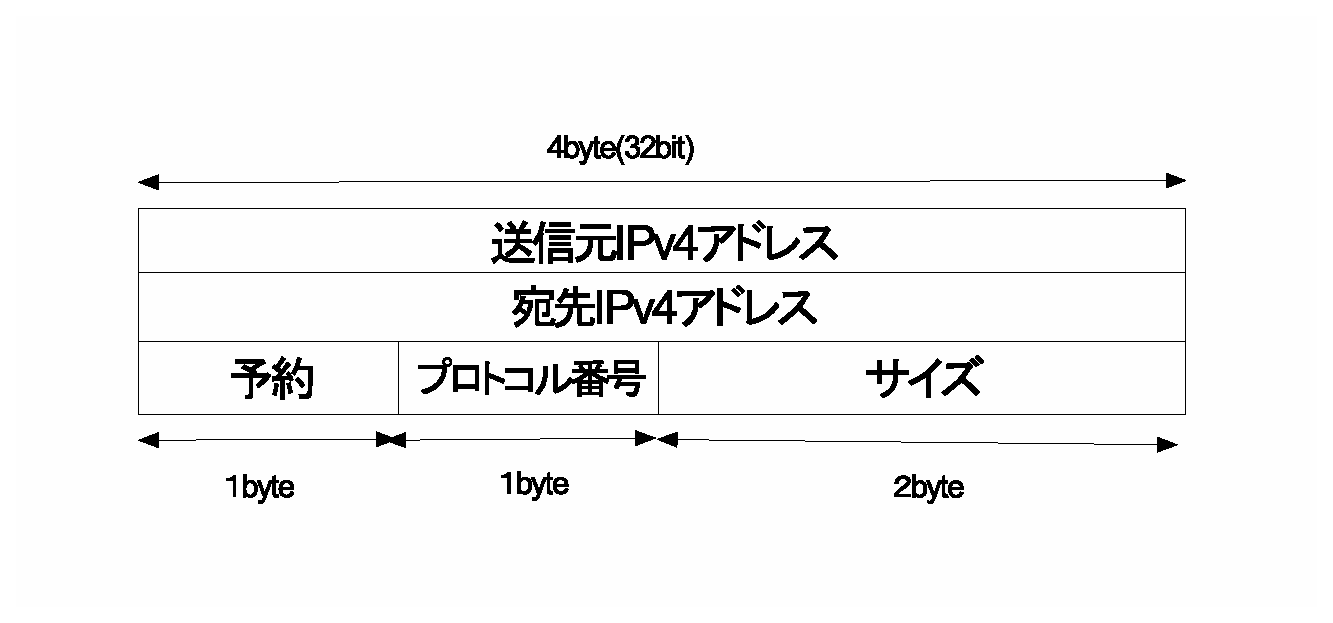
\includegraphics[width=12cm,clip]{draw/pseudoheader4.eps}
	\caption{インターネットプロトコル層がIPv4の疑似ヘッダの構造}
	\label{fig:pseudo}
\end{figure}

図\ref{fig:pseudo}は、インターネットプロトコル層がIPv4の疑似ヘッダである。

発信元IPアドレス、宛先IPアドレス、プロトコル、データ長の各フィールドで構成されている。プロトコルフィールドはTCPであれば6,UDPであれば17が入る。また、データ長フィールドには、疑似ヘッダを除く、実在するヘッダとデータ部分の長さの合計が入る。

\subsection{IPv6の疑似ヘッダ}

\begin{figure}[htbp]
	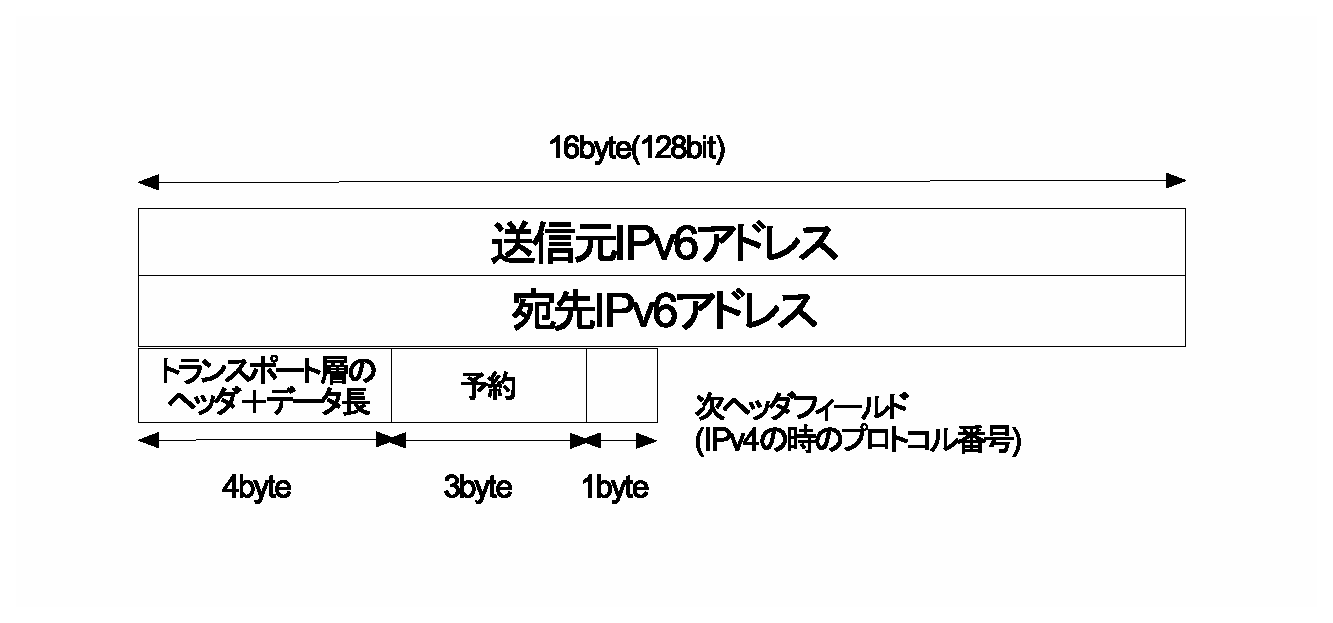
\includegraphics[width=12cm,clip]{draw/pseudoheader6.eps}
	\caption{インターネットプロトコル層がIPv6のときの疑似ヘッダの構造}
	\label{fig:pseudo6}
\end{figure}

図\ref{fig:pseudo6}は、インターネットプロトコル層がIPv6の疑似ヘッダである。

基本的な構造、内包するデータはIPv4の場合とほぼ同様である。IPv6のデータグラムは、ジャンボグラム拡張と呼ばれる拡張で、最大4GiBまでの大きさを採ることができる。そのため、サイズは32bit(4byte)となっている。予約フィールドのビットは全て0である。

また、プロトコル番号に層等するフィールドは、ネクストヘッダ番号となっている。ネクストヘッダ番号の番号自体はIPv4のプロトコル番号なので、IPv4の時と同様に、TCPなら6、UDPなら17が入る。

UDPならびにTCPでは疑似ヘッダをどう使用しているか、それぞれの章での解説で改めて説明する。

